\documentclass[11pt]{article}
\usepackage{graphicx}
\usepackage[utf8]{inputenc}
\usepackage{enumerate}
\usepackage{multirow,tabularx}
\usepackage{caption}
\usepackage{subfigure}
\usepackage[T1]{fontenc}
\usepackage{mathptmx}
\usepackage[a4paper, left=2cm, right=2cm, top=2.5cm, bottom=2.5cm, headsep=1.2cm]{geometry} 
\usepackage[rightcaption]{sidecap}
\usepackage{float}
\usepackage{pgfplots}
\pgfplotsset{compat=1.14}
\begin{document}

\begin{titlepage}

	\begin{center}

    


	\huge{\textsc{Metody Komputerowe w Spalaniu}} \\
[10mm]

    \LARGE{\textbf{Autoignition of a methane air mixture at stoichiometry, for different initial temperature and initial pressure
}} \\
	[50mm]
	\Large{Mateusz Klos}\\
    \Large{271313}\\
    [25mm]
    \large{Aerospace Engineering}\\
    [3mm]
    \large{Warsaw, 26.04.2017}\\
    \end{center}
    
\end{titlepage}

\newpage



\section{Purpose of the project}
The purpose of the project is to conduct a study of autoignition of a ethane - air mixture at stoichiometry for different initial temperature, pressure. The task is to find relationship between initial conditions and autoignition timing. I used Cantera, an open-source chemical kinetics software.


Combustion reaction of ethane - air mixture at stoichiometry:
\begin{displaymath}
C_{2}H_{6} + 3.5 (O_{2} + 3.76 N_{2}) \Rightarrow 2 CO_{2} + 6 H_{2}O + 13.16 N_{2}
\end{displaymath}

\section{Mathematical model}
To find autoignition time I used the gradient method. The time of the sharpest temperature increase is the autoignition point. In order to catch this point, the step of the simulation was set to - 10{$^{-5}$} sec. The calculations were held for 6 different temperatures and 6 different values of pressure. 

\section{Results and plots}

\subsection{Results for Ti=1000K and different initial pressure.}
\begin{figure} [H]
	\begin{center}
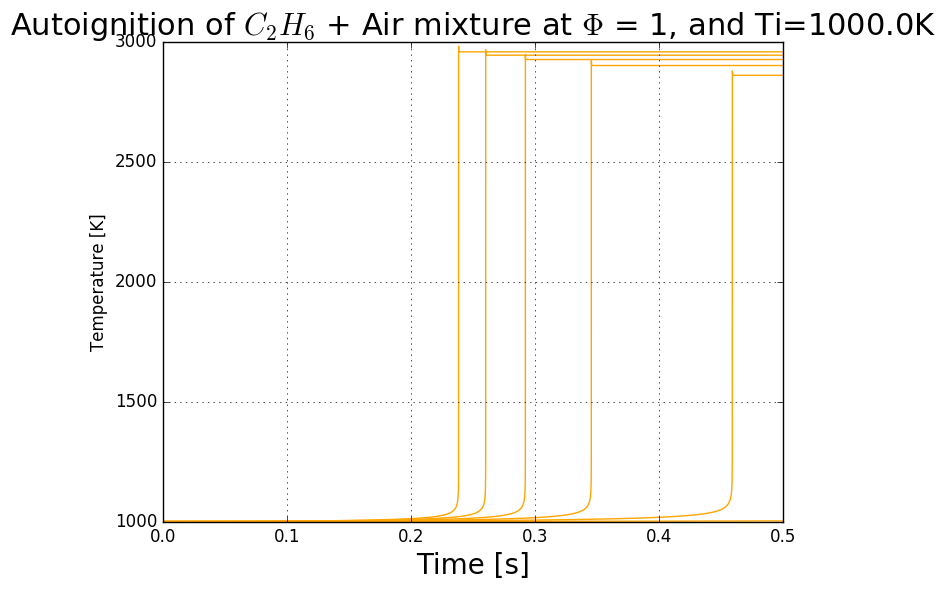
\includegraphics[height=0.5\textwidth]{T5_T_Trange_UV}
        \caption{Influence of initial pressure on temperature change over time.}
    \end{center}
\normalsize
{The autoignition timing decreases as initial pressure rises. This graph shows also that higher initial pressure causes higher final temperature. After autoignition temperature rises rapidly and then slightly drops and stabilizes.}
\end{figure}

\begin{figure} [H]
	\begin{center}
    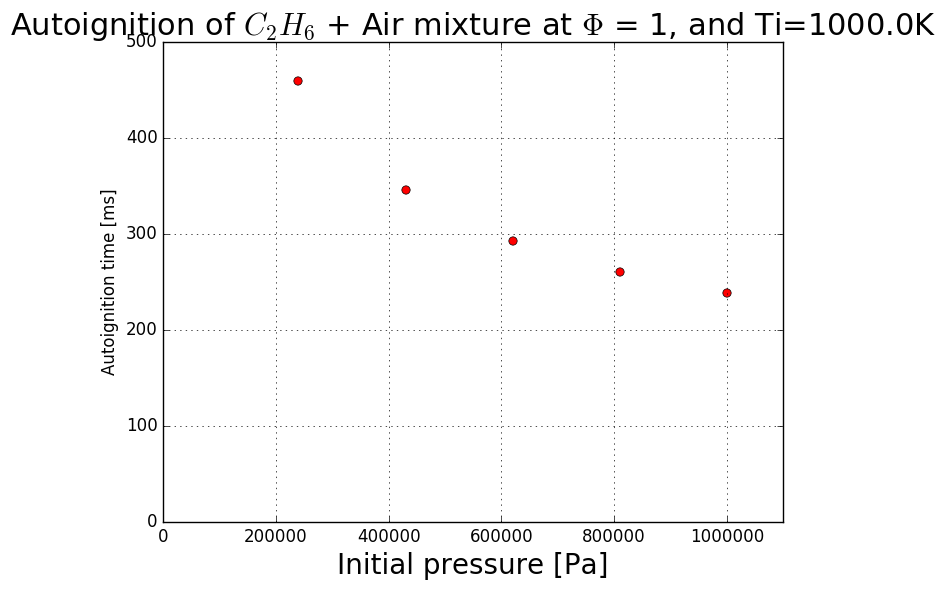
\includegraphics[height=0.5\textwidth]{T5_Autoignition}
        \caption{Influence of initial pressure on autoignition timing.}
    \end{center}
\normalsize
{This graph shows that autoignition time is lower for higher pressure.}
\end{figure}

\subsection{Results for P=50kPa and different initial temperatures}
\begin{figure} [H]
	\begin{center}
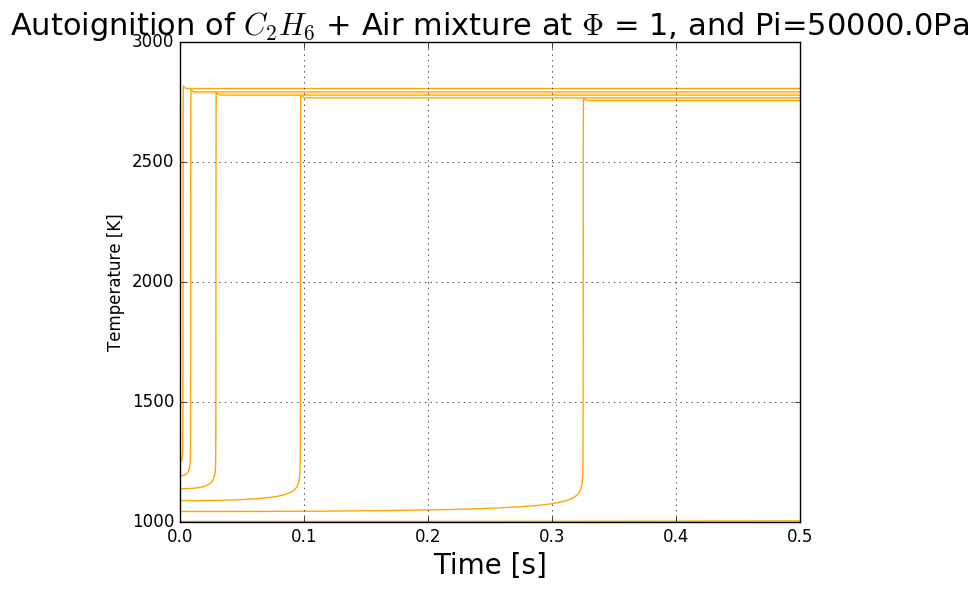
\includegraphics[height=0.5\textwidth]{P0_T_Trange_UV}
        \caption{Influence of initial temperature on temperature change over time.}
    \end{center}
\normalsize
{Lower initial temperature gives lower final temperature.}
\end{figure}

\begin{figure} [H]
	\begin{center}
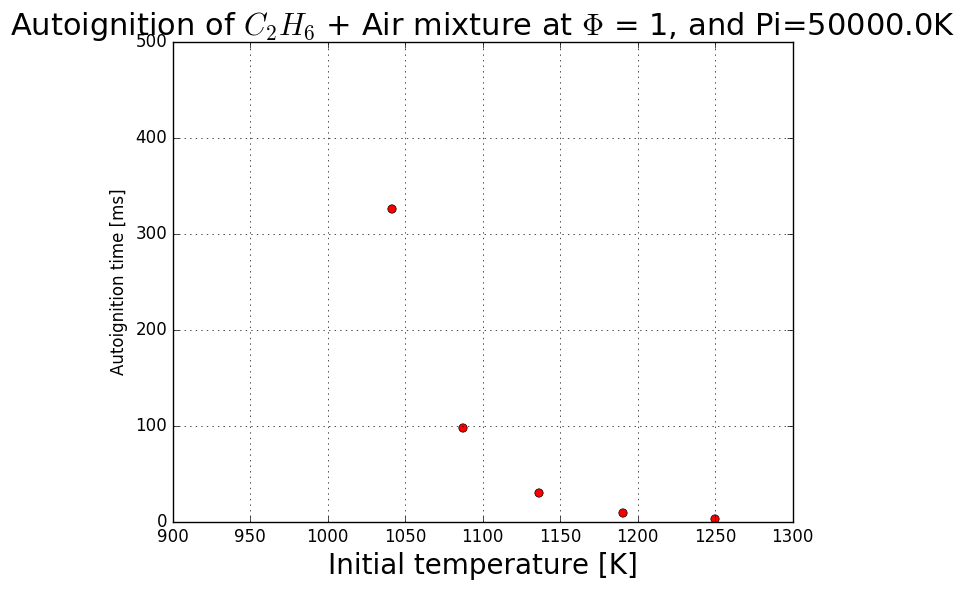
\includegraphics[height=0.5\textwidth]{P0_Autoignition}
        \caption{Influence of initial temperature on autoignition timing.}
    \end{center}
\normalsize
{The autoignition timing decreases for greater values of temperature.}
\end{figure}




\section{Conclusion}
The study gives information about the behavior of autoignition with different initial conditions. Both increased temperature and pressure shorten ignition time and increase final temperature. More data (relationship between 6 temperatures, 6 values of pressure and autoignition timing) are located in the .csv file.

Three dimensional representation of received data:
\begin{center}
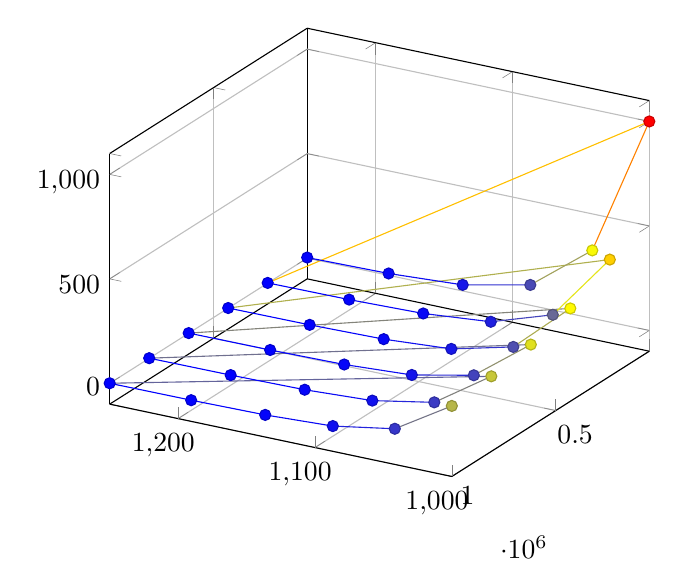
\begin{tikzpicture}
	\begin{axis}[grid=major,view={210}{30}]
	\addplot3+[mesh,scatter,samples=36] 
		coordinates {
(1250.0,50000.0,2.665)
(1190.47619048,50000.0,8.785)
(1136.36363636,50000.0,29.195)
(1086.95652174,50000.0,97.315)
(1041.66666667,50000.0,325.365)
(1000.0,50000.0,999.994999998)
(1250.0,240000.0,1.125)
(1190.47619048,240000.0,3.695)
(1136.36363636,240000.0,12.265)
(1086.95652174,240000.0,40.955)
(1041.66666667,240000.0,136.975)
(1000.0,240000.0,458.915)
(1250.0,430000.0,0.855)
(1190.47619048,430000.0,2.805)
(1136.36363636,430000.0,9.305)
(1086.95652174,430000.0,30.965)
(1041.66666667,430000.0,103.255)
(1000.0,430000.0,345.245)
(1250.0,620000.0,0.735)
(1190.47619048,620000.0,2.395)
(1136.36363636,620000.0,7.915)
(1086.95652174,620000.0,26.255)
(1041.66666667,620000.0,87.405)
(1000.0,620000.0,292.065)
(1250.0,810000.0,0.655)
(1190.47619048,810000.0,2.145)
(1136.36363636,810000.0,7.065)
(1086.95652174,810000.0,23.405)
(1041.66666667,810000.0,77.825)
(1000.0,810000.0,260.045)
(1250.0,1000000.0,0.605)
(1190.47619048,1000000.0,1.965)
(1136.36363636,1000000.0,6.475)
(1086.95652174,1000000.0,21.445)
(1041.66666667,1000000.0,71.275)
(1000.0,1000000.0,238.215)
};
	\end{axis}
\end{tikzpicture}
\end{center}
\newpage

\section{References}
\begin{enumerate}
	\item{CANTERA\_HandsOn.pdf}
    \item{Wyklad\_4\_Cantera.pdf}
\end{enumerate}










\end{document}